\chapter{Introduction}
\label{c:intro}

\note{Introductory text goes here!}

This paper introduces a family of algorithms for finding maximum common
substructures in a broad class of objects that includes both graphs and
hypergraphs.

\section{Maximum Common Induced Subgraph}

We begin with a well-known problem: maximum common induced subgraph (MCIS). A
graph $G$ is a pair $(V, E)$, where $V = V(G)$ is the vertex set and $E = E(G)$
is the edge set. Each element of $E$ is a two-element subset of $V$, whose
elements are referred to as its endpoints. For example, we may have
\[
V = \{1, 2, 3, 4, 5, 6\},
E = \{\{1,2\}, \{1,3\}, \{2,3\}, \{3,4\}, \{4,5\}, \{4,6\}, \{5,6\}\}
.
\]
This graph may be drawn as shown in \Cref{fig:introA}, with a point for each
vertex and a line for each edge.  The positions of the points in the plane have
no significance.

\begin{figure}[h!]
\centering
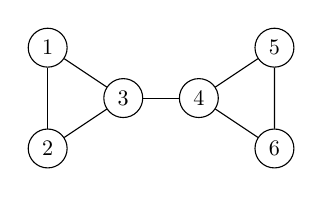
\begin{tikzpicture}[scale=0.8, every node/.style={scale=0.8}]
%\begin{tikzpicture}
  \node [draw,circle] (1) at (0,1.6) {1};
  \node [draw,circle] (2) at (0,0) {2};
  \node [draw,circle] (3) at (1.2,.8) {3};
  \node [draw,circle] (4) at (2.4,.8) {4};
  \node [draw,circle] (5) at (3.6,1.6) {5};
  \node [draw,circle] (6) at (3.6,0) {6};
  \draw (1) -- (2);
  \draw (1) -- (3);
  \draw (2) -- (3);
  \draw (3) -- (4);
  \draw (4) -- (5);
  \draw (4) -- (6);
  \draw (5) -- (6);
\end{tikzpicture}
\caption{A graph}
\label{fig:introA}
\end{figure}

Two graphs are isomorphic if they can be drawn identically. Thus, the graph in
Figure B is isomorphic to the graph in \Cref{fig:introA}, despite having a different
vertex set. Formally, an isomorphism between graphs $G$ and $H$ is a bijection $f$
between the vertex set of $G$ and the vertex set of $H$, such that if we apply $f$ to
the endpoints of each edge of $G$ we obtain the edge set of $H$. If such an $f$
exists, we say that $G$ and $H$ are isomorphic.

\begin{figure}[h!]
\centering
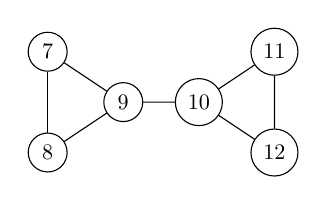
\begin{tikzpicture}[scale=0.8, every node/.style={scale=0.8}]
%\begin{tikzpicture}
  \node [draw,circle] (1) at (0,1.6) {7};
  \node [draw,circle] (2) at (0,0) {8};
  \node [draw,circle] (3) at (1.2,.8) {9};
  \node [draw,circle] (4) at (2.4,.8) {10};
  \node [draw,circle] (5) at (3.6,1.6) {11};
  \node [draw,circle] (6) at (3.6,0) {12};
  \draw (1) -- (2);
  \draw (1) -- (3);
  \draw (2) -- (3);
  \draw (3) -- (4);
  \draw (4) -- (5);
  \draw (4) -- (6);
  \draw (5) -- (6);
\end{tikzpicture}
\caption{Figure B TODO: add caption}
\end{figure}

An induced subgraph of $G = (V, E)$ has a subset $W$ of $V$ as its vertex set, and
$\{\{u, v\} \in E \mid u, v \in W\}$ as its edge set; that is, the subgraph
includes all edges of $G$ both of whose endpoints appear in $W$.  The first graph
in Figure C is thus an induced subgraph of the graph in Figure A, whereas the
second graph is not. We say that the set $W$ induces the subgraph.

\begin{figure}[h!]
\centering
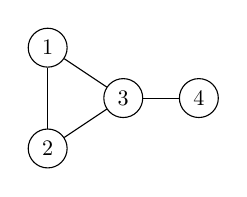
\begin{tikzpicture}[scale=0.8, every node/.style={scale=0.8}]
  \node [draw,circle] (1) at (0,1.6) {1};
  \node [draw,circle] (2) at (0,0) {2};
  \node [draw,circle] (3) at (1.2,.8) {3};
  \node [draw,circle] (4) at (2.4,.8) {4};
  \draw (1) -- (2);
  \draw (1) -- (3);
  \draw (2) -- (3);
  \draw (3) -- (4);
\end{tikzpicture}
\qquad
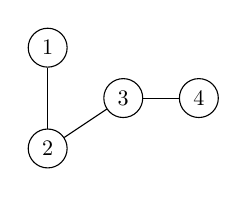
\begin{tikzpicture}[scale=0.8, every node/.style={scale=0.8}]
  \node [draw,circle] (1) at (0,1.6) {1};
  \node [draw,circle] (2) at (0,0) {2};
  \node [draw,circle] (3) at (1.2,.8) {3};
  \node [draw,circle] (4) at (2.4,.8) {4};
  \draw (1) -- (2);
  \draw (2) -- (3);
  \draw (3) -- (4);
\end{tikzpicture}
\caption{Figure C TODO: add caption}
\end{figure}

A \emph{common induced subgraph} of graphs $G$ and $H$ is an induced subgraph of $G$ which
is isomorphic to an induced subgraph of $H$. In figure D, a common induced
subgraph of the two graphs is shown in bold on the first graph, and its
isomorphic subgraph is shown in bold on the second graph.

\begin{figure}[h!]
\centering
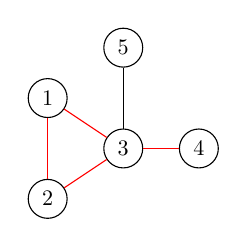
\begin{tikzpicture}[scale=0.8, every node/.style={scale=0.8}]
  \node [draw,circle] (1) at (0,1.6) {1};
  \node [draw,circle] (2) at (0,0) {2};
  \node [draw,circle] (3) at (1.2,.8) {3};
  \node [draw,circle] (4) at (2.4,.8) {4};
  \node [draw,circle] (5) at (1.2,2.4) {5};
  \draw [red] (1) -- (2);
  \draw [red] (1) -- (3);
  \draw [red] (2) -- (3);
  \draw [red] (3) -- (4);
  \draw (3) -- (5);
\end{tikzpicture}
\qquad
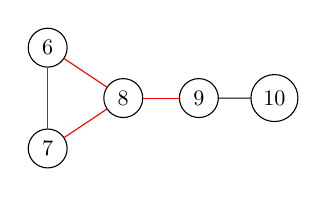
\begin{tikzpicture}[scale=0.8, every node/.style={scale=0.8}]
  \node [draw,circle] (1) at (0,1.6) {6};
  \node [draw,circle] (2) at (0,0) {7};
  \node [draw,circle] (3) at (1.2,.8) {8};
  \node [draw,circle] (4) at (2.4,.8) {9};
  \node [draw,circle] (5) at (3.6,.8) {10};
  \draw [red] (1) -- (2);
  \draw [red] (1) -- (3);
  \draw [red] (2) -- (3);
  \draw [red] (3) -- (4);
  \draw (4) -- (5);
\end{tikzpicture}
\caption{Figure D TODO: add caption}
\end{figure}

A maximum common induced subgraph of $G$ and $H$ is a common induced subgraph of $G$
and $H$ such that no common induced subgraph of the two graphs has a larger
vertex set.

\section{Maximum Common Induced Sub-Hypergraph}

We now describe a problem that includes MCIS as a special case: \emph{maximum common
induced sub-hypergraph (MCISH)} \cite{DBLP:series/sci/BunkeDKNS08}. The class of
\emph{hypergraphs} extends the class of graphs by permitting edges containing more
than two vertices. For example, the hypergraph $(\{1,2,3,4,5\}, \{\{1,2,3\}, \{1,4\}\})$
is shown in Figure E; each edge is shown as a shape enclosing two or more
vertices.

\begin{figure}[h!]
\centering
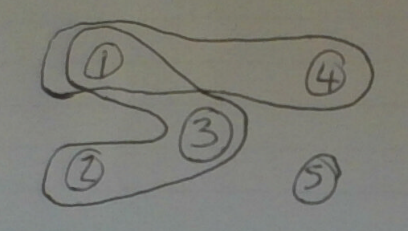
\includegraphics[width=0.5\textwidth]{10-introduction/img/figureE}
\caption{Figure E TODO: add caption}
\end{figure}

As with graphs, an isomorphism is a bijection between vertex sets that
preserves edges sets, and two hypergraphs are said to be isomorphic if there is
an isomorphism between their vertex sets.

\emph{Induced sub-hypergraph} is defined analogously to induced subgraph.  Let $G=(V,E)$
be a hypergraph, and $W$ be a subset of $V$. Then the sub-hypergraph of $G$ induced
by $W$ has $W$ as its vertex set, and its edge set contains each element of $E$ whose
members are all in $W$. As an example, the sub-hypergraph of the hypergraph in
Figure E induced by $\{1,2,3,5\}$ is $(\{1,2,3,5\}, \{\{1,2,3\}\})$.

A \emph{common induced sub-hypergraph (CISH)} of hypergraphs $G$ and $H$ is an induced
sub-hypergraph of $G$ which is isomorphic to an induced sub-hypergraph of $H$. A
maximum common induced sub-hypergraph is a CISH with as many vertices as
possible.

\section{Maximum Common Induced Subgraph for Directed Graphs}

The maximum common induces subgraph problem for directed graphs (MCIS-D) is the
directed-graph analogue of MCIS.  A directed graph is a pair $(V,A)$, where $V$ is
the vertex set and $A$, a set of ordered pairs of elements of $V$, is the arc set.
As an example, Figure F shows the directed graph $(\{1,2,3\}, \{(1,2), (2,1),
(2,3)\})$.

\begin{figure}[h!]
\centering
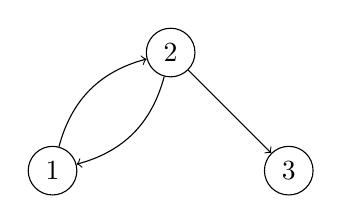
\begin{tikzpicture}[->]
%\begin{tikzpicture}
  \node [draw,circle] (1) at (0,0) {1};
  \node [draw,circle] (2) at (1.5,1.5) {2};
  \node [draw,circle] (3) at (3,0) {3};
  \draw[->,bend left=30] (1) edge (2);
  \draw[->,bend left=30] (2) edge (1);
  \draw (2) -> (3);
\end{tikzpicture}
\caption{Figure F TODO: add caption}
\end{figure}

For edge $(u,v)$, we say that $u$ is the source vertex and $v$ is target vertex; both
$u$ and $v$ are called endpoints.

Subgraph, isomorphism, and maximum common induced subgraph are defined
analogously to the undirected version.

\section{Generalised Maximum Common Induced Subgraph}

We now introduce a problem that generalises all three of the problems discussed
so far. We introduce the concept of a \emph{generalised graph (g-graph)}. A
g-graph $G = (V, E)$ has a vertex set $V$ and edge set $E$. Each edge in $E$ is
non-empty tuple of non-empty subsets of $V$. An example of a g-graph with five
vertices and three edges is
\[
(\{1,2,3,4,5\}, \{(\{1,2\},\{4\}), (\{1,2\}), (\{3\},\{4\})\}).
\]

If we restrict elements of E to be 1-tuples of 2-element sets, then g-graphs
are equivalent to graphs. If we remove the upper bound on set size, g-graphs
become equivalent to hypergraphs. If instead we restrict elements of E to be
2-tuples of singleton sets, then g-graphs are equivalent to directed graphs.

G-graphs can model other types of object such as directed hypergraphs \cite{DBLP:journals/dam/GalloLP93} and a generalisation of directed graphs
where each edge may be a path of two or more vertices.

Isomorphism and induced subgraph are defined analogously to their graph
versions. We call the MCIS problem on g-graphs generalised maximum common
induced subgraph (G-MCIS).

\section{Maximum Common Edge Subgraph Problems}

We now consider the \emph{maximum common edge subgraph (MCES)} family of problems,
beginning with the simple case of undirected graphs. An edge subgraph of $(V, E)$
is any graph $(W, F)$ such that $W$ is a subset of $V$ and $F$ is a subset of $E$; the
subgraph may thus contain any subsets of the vertices and edges of the original
graph, as long as the subgraph’s vertex set contains all of the endpoints of
edges in its edge set. To give two examples, both graphs in Figure C are edge
subgraphs of the graph in Figure B. Every induced subgraph of a graph $G$ is also
an edge subgraph of $G$.

A common edge subgraph of graphs $G$ and $H$ is an edge subgraph of $G$ that is
isomorphic to an edge subgraph of $H$. A maximum common edge subgraph of two
graphs is a common edge subgraph with as many edges as possible.

?? Chemistry application

We can extend the definition of MCES to g-graphs to give the G-MCES problem.
Analogously to its induced counterpart, this has maximum common edge subgraph
in directed graphs and maximum common edge sub-hypergraph as special cases.

\section{Variants}

Maximum common subgraph problems may be extended by associating a label
function with each graph, which maps each vertex and each edge to a value. The
isomorphism between subgraphs is required to be label-preserving.

?? Loops

\section{Related Problems}

MCIS generalises the induced subgraph isomorphism problem, which is the problem
of determining whether graph $G$ is isomorphic to an induced subgraph of graph $H$.
MCES generalises the non-induced subgraph isomorphism problem, which is to
determine whether $G$ is isomorphic to an edge subgraph of $H$. Both problems are
NP-complete; thus, all of the maximum common subgraph problems described so far
are NP-hard.

Both of the subgraph isomorphism problems generalise graph isomorphism, which
is to determine whether two graphs are isomorphic. ?? As we will discuss later,
our partitioning algorithms have similarities to graph isomorphism algorithms
such as Conauto.

The maximum clique problem is to find an induced subgraph of a graph $G$ with as
many vertices as possible, such that the subgraph has all possible edges; that
is ??. Maximum clique can be solved (although rather inefficiently in practice)
using an MCIS algorithm, by finding the MCIS of $G$ and a complete graph with the
same number of vertices as $G$.

\section{Existing Algorithms}

In this subsection, we outline the existing approaches for solving MCIS on
undirected graphs. Algorithms for other maximum common subgraph problems have
similarities to these approaches, and will be described in detail in later
chapters.

It is useful to introduce the concept of a mapping to denote a pair of common
subgraphs of input graphs $G$ and $H$ and the isomorphism between these subgraphs.
A mapping $M$ is a set of 2-tuples, where each tuple contains a vertex from the
first graph followed by a vertex from the second graph. The subgraph of $G$ is
induced by $\{u \mid (u, v) \in M\}$, and the subgraph of $H$ is induced by $\{v \mid (u, v)
\in M\}$. The isomorphism between these subgraphs is a function that maps each $u$
that appears as the first element of a 2-tuple to the second element of that
tuple.

The association graph of $G$ and $H$ is a graph with $\{(u,v) \mid u \in V(G) \wedge v \in
V(H)\}$ as its vertex set; it thus has $|V(G)||V(H)|$ vertices. Two vertices $(u,v)$
and $(u',v')$ in the association graph are adjacent if and only if all of the
following conditions are met.

\begin{itemize}
  \item $u \not= u'$
  \item $v \not= v'$
  \item $((u,u') \in E(G)) = ((v,v') \in E(H))$
\end{itemize}

A subset of the vertices of the association graph is a valid mapping if and
only if it is a clique in the association graph (?? proof?). Thus, we can find
an MCIS of G and H by running a maximum clique solver on the association graph
of G and H. Association graph encodings can be used to solve directed MCIS on
directed graphs and (with modifications) MCES. However, they cannot be used to
solve more complex variants such as maximum common induced sub-hypergraph.
(Although it might be possible to solve such problems by devising an
association hypergraph, we do not consider this possibility further.)

\section{Backtracking Search}

TODO: describe search tree, CP, forward checking, levels of consistency.

\section{Branch and Bound}

All of the maximum common subgraph problems discussed in this paper are
optimisation problems.  Branch and bound is a general technique for solving
optimisation problems by backtracking search. We will describe branch and bound
in the context of maximisation (rather than minimisation) problems.

During search, we maintain an incumbent---the best solution found so far. Each
time a solution $S$ whose objective value is larger than the incumbent is found,
the incumbent’s value is updated to $S$. At each search node we calculate an
upper bound on the best objective value that can be obtained by extending the
current partial solution. If this upper bound is not greater than the
incumbent’s objective value, we know that exploring the subtree below the
current search node would be fruitless, and we therefore backtrack.

An alternative to branch and bound is to solve the maximisation problem by a
sequence of decision problems. Beginning at a known upper bound $B$ for the
optimal objective value, we use search to answer the question “does a solution
with objective value B exist?” If the answer is “yes”, the algorithm
terminates. Otherwise, a solution with objective value $B-1$ is sought, then $B-2$,
and so on until a solution is found.

A third alternative for solving optimisation problems, which again involves a
sequence of decision problems, is binary search on the objective value. Begin
with a known lower bound $L$ and a known upper bound $B$ for the objective value.
(For MCIS, we could trivally use $L=0$ and $B=|V(G)|$.) ?? Then do binary search to
find the largest objective value for which the decision problem is satisfiable.
Cite the book cited in the Handbook of CP. Say why we don’t try this approach
in this thesis.  Say what this approach would gain us.

\section{Inexact Algorithms}

TODO

\section{New algorithms in this thesis}

The McSplit family of algorithms has branch-and-bound variants and variants
that use a sequence of decision problems; it also has variants for induced and
edge subgraph problems. The summary in this section discusses only the induced
variants.

McSplit performs tree search in the style of a forward-checking constraint
programming algorithm. Rather than maintaining an explicit domain for each
vertex in the first graph, vertices are re-labelled at each search node in such
a way that the current mapping may only be extended by mapping a vertex in
first graph to a vertex in the second graph with the same label. Labels may be
viewed as equivalence classes of vertices, and at each search node these
classes are refined (partitioned) into smaller classes. We store the vertices
of each graph as a list (without copying at each search node), and can perform
this partitioning efficiently be re-arranging the vertices in each list. This
data structure makes it possible to calculate an upper bound very cheaply at
each search node, and permits the cheap computation of good variable-ordering
heuristics.

\section{Structure of the Dissertation}

Chapter 2 surveys the literature on algorithms for MCIS, MCES, and related
problems. Chapter 3 introduces the McSplit algorithm for MCIS on undirected
graphs. Chapter 4 generalises McSplit to MCIS problems on g-graphs. In Chapter
5, we turn to MCES, and describe how this can be solved by a variant of McSplit
and by association graph encodings. In Chapter 6, we introduce a variant of
McSplit for block and bridge preserving MCIS, a version of the problem with
applications to chemistry. Chapter 7 concludes.

%==============================================================================
\section{Thesis Statement}
\label{c:intro:thesisstatement}

TODO

